% Dynamic inverse-$\varGamma$-equivalent circuit for an induction machine
% Author: Erno Pentzin (2013)
\documentclass[12pt]{standalone}
\usepackage{tikz}
\usepackage[americanresistors,americaninductors]{circuitikz}
\usepackage{graphicx,subfig}
\usetikzlibrary{positioning}
\usetikzlibrary{arrows}
\usepackage[export]{adjustbox}
\usepackage{floatrow}

\newsavebox{\axes}
\sbox{\axes}
{
\begin{tikzpicture}[overlay]
  % origin point
  \draw [color=black, fill=black] (0, 0) circle (0.1);
  \draw [color=black, fill=none] (0, 0) circle (0.2);
  % x-axis
  \draw [line width=0.25mm] (0, 0) -- (5, 0);
  % y-axis
  % x-axis label
  \node at (4.5, 0.25) {$k_x$};
  % y-axis label
  \node at (0.25, 4.5) {$k_y$};
  \draw [line width=0.25mm] (0, 0) -- (0, 5);
  % unit x-axis
  \draw [line width=0.45mm,->] (0, 0) -- (2, 0);
  % unit y-axis
  \draw [line width=0.45mm,->] (0, 0) -- (0, 2);
  % origin label
  \node at (-0.25, -0.25) {$\mathbf{\hat z}$};
  % Unit x-axis label
  \node at (1.5, -0.2) {$\mathbf{\hat x}$};
  % Unit y-axis label
  \node at (-0.2, 1.5) {$\mathbf{\hat y}$};
\end{tikzpicture}
}

\newsavebox{\isource}
\sbox{\isource}
{%
\begin{circuitikz}[overlay]
  \draw
  (7,2.5) to[american current source] (12,2.5);
\end{circuitikz}
}

\newsavebox{\vsource}
\sbox{\vsource}
{%
\begin{circuitikz}[overlay]
  \draw[line width=0.25mm]
  (7,2.5) to[american voltage source] (12,2.5);
\end{circuitikz}
}


\begin{document}
  \minipage{1.08\textwidth}
  \begin{figure}[tbh]
    \centering
    % \begin{adjustbox}{scale=0.6}
    \begin{subfloatrow}
      \sidesubfloat{
      \begin{tikzpicture}
        % Draw coordinate system
        \usebox {\axes}
        % Source and label (use arrows command to insert arrow of choice)
        \draw [line width=0.5mm,arrows={-latex}] (2, 2) -- (3, 2);
        \node at (2.5, 2.5) {${\tilde{J}_x}$};
        % Draw the equivalent TL
        \draw[line width=0.25mm] (7,0) -- (7,5);
        \draw[line width=0.25mm] (12,0) -- (12,5);
        % Insert Source
        \usebox {\isource}
      \end{tikzpicture}
      }
    \end{subfloatrow}
    \vspace{1cm}
    \begin{subfloatrow}
      \sidesubfloat{
      \centering
      \begin{tikzpicture}
        % Draw coordinate system
        \usebox {\axes}
        % Source and label (use arrows command to insert arrow of choice)
        \draw [line width=0.5mm,arrows={-latex}] (2, 2) -- (2, 3);
        \node at (2.5, 2.5) {${\tilde{J}_y}$};
        % Draw the equivalent TL
        \draw[line width=0.25mm] (7,0) -- (7,5);
        \draw[line width=0.25mm] (12,0) -- (12,5);
        % Insert Source
        \usebox {\isource}
      \end{tikzpicture}
      }
    \end{subfloatrow}
    \vspace{1cm}
    \begin{subfloatrow}
      \sidesubfloat{
      \centering
      \begin{tikzpicture}
        % Draw coordinate system
        \usebox {\axes}
        % Source and label (use arrows command to insert arrow of choice)
        \draw [line width=0.5mm,arrows={-latex}] (2, 2) -- (2, 3);
        \node at (2.5, 2.5) {${\tilde{J}_y}$};
        % Draw the equivalent TL
        \draw[line width=0.25mm] (7,0) -- (7,5);
        \draw[line width=0.25mm] (12,0) -- (12,5);
        % Insert Source
        \usebox {\isource}
      \end{tikzpicture}
      }
    \end{subfloatrow}
    \vspace{1cm}
    \begin{subfloatrow}
      \sidesubfloat{
      \centering
      \begin{tikzpicture}
        % Draw coordinate system
        \usebox{\axes}
        % Source and label (use arrows command to insert arrow of choice)
        \draw [line width=0.5mm,arrows={-latex}] (2, 2) -- (2, 3);
        \node at (2.5, 2.5) {${\tilde{J}_y}$};
        % Draw the equivalent TL
        \draw[line width=0.25mm] (7,0) -- (7,5);
        \draw[line width=0.25mm] (12,0) -- (12,5);
        % Insert Source
        \usebox {\isource}
      \end{tikzpicture}
      }
    \end{subfloatrow}
    % \end{adjustbox}
  \end{figure}
  \endminipage
\end{document}
